% ============================================
% METHODOLOGY
% ============================================

\begin{frame}{Methodology -- Current 4-Stage Pipeline}
    \begin{center}
        
\includegraphics[width=\textwidth,height=0.74\textheight,keepaspectratio]{src/images/fiximag.png}
    \end{center}
\end{frame}

% ============================================
% AGENT 1
% ============================================
\begin{frame}{Agent 1 -- Raw Structural Profiler}
    \begin{columns}[T]
        \begin{column}{0.55\textwidth}
            \begin{itemize}
                \item Reads the input CSV and records shape, dtypes, missingness, uniqueness, and duplicates.
                \item Produces a raw structural profile without changing the source data.
                \item Caches the DataFrame for the downstream stages.
            \end{itemize}
        \end{column}
        \begin{column}{0.42\textwidth}
            \centering
            
\includegraphics[width=\linewidth,height=0.80\textheight,keepaspectratio]{src/images/agent1pic.png}
        \end{column}
    \end{columns}
\end{frame}

% ============================================
% AGENT 2
% ============================================
\begin{frame}{Agent 2 -- Technical Inference \& Semantic Tagging}
    \begin{columns}[T]
        \begin{column}{0.55\textwidth}
            \begin{itemize}
                \item Sniffs numeric, datetime, boolean, and string types using local heuristics.
                \item Uses Groq-based semantic tagging when available and falls back to deterministic rules when it is not.
                \item Creates a per-column blueprint containing type, semantic tag, scaling, imputation, and analysis policies.
                \item Passes the blueprint to preprocessing instead of hard-coding one rule for every column.
            \end{itemize}
        \end{column}
        \begin{column}{0.42\textwidth}
            \centering
            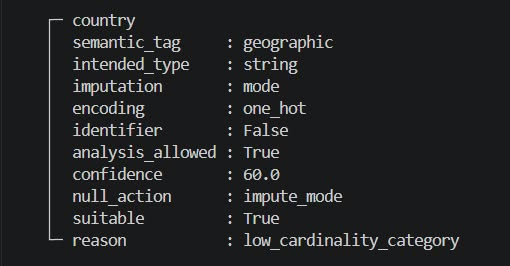
\includegraphics[width=\linewidth,keepaspectratio]{src/images/agent2pic.png}
        \end{column}
    \end{columns}
\end{frame}

% ============================================
% AGENT 3
% ============================================
\begin{frame}{Agent 3 -- Context-Aware Preprocessing}
    \begin{columns}[T]
        \begin{column}{0.55\textwidth}
            \begin{itemize}
                \item Coerces columns according to the semantic blueprint and cleans international currency formats.
                \item Standardizes text and null variants while preserving identifiers.
                \item Removes duplicates, applies configured imputation, and clips permitted outliers with IQR bounds.
                \item Extracts date features and derives metrics such as profit, margin, and revenue per unit.
                \item Records scaling parameters, an audit log, and a 0--100 data quality score.
            \end{itemize}
        \end{column}
        \begin{column}{0.42\textwidth}
            \centering
            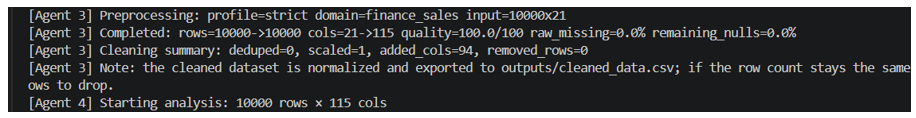
\includegraphics[width=\linewidth,height=0.80\textheight,keepaspectratio]{src/images/agent3pic.png}
        \end{column}
    \end{columns}
\end{frame}

% ============================================
% AGENT 4
% ============================================
\begin{frame}{Agent 4 -- Visualization \& Statistical Analysis}
    \begin{columns}[T]
        \begin{column}{0.55\textwidth}
            \begin{itemize}
                \item Calculates descriptive statistics, correlations, distributions, growth, and seasonality.
                \item Detects anomalies using a configurable z-score threshold.
                \item Computes regression trends and category rankings when the dataset supports them.
                \item Saves reproducible PNG charts and structured statistics to the pipeline state.
            \end{itemize}
        \end{column}
        \begin{column}{0.42\textwidth}
            \centering
            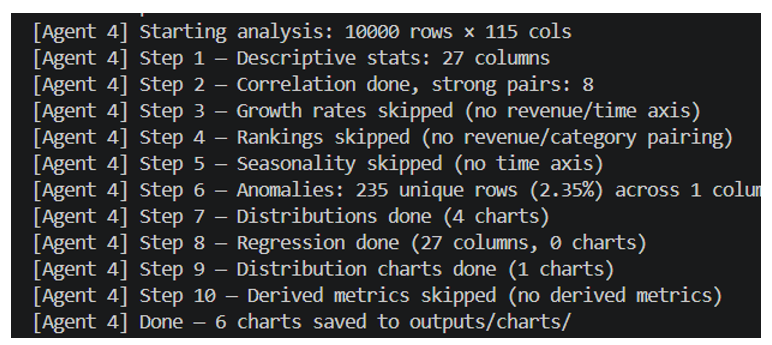
\includegraphics[width=\linewidth,keepaspectratio]{src/images/agent4pic.png}
        \end{column}
    \end{columns}
\end{frame}

% ============================================
% AGENT 5
% ============================================
